% By zmienic jezyk na angielski/polski, dodaj opcje do klasy english lub polish
\documentclass[polish, 12pt]{aghthesis}
\usepackage{babel}
\usepackage[utf8]{inputenc}
\usepackage{url}
\usepackage{indentfirst}
\usepackage{amsmath}
\usepackage{graphicx}
\usepackage{caption}
\usepackage{subcaption}
\usepackage{listings}

\author{Dawid Romanowski, Wojciech Czarny}

\title{Implementacja metody SPH \\ na procesory graficzne}

\supervisor{dr hab. inż. Krzysztof Boryczko, prof. nadzw. AGH}

\date{2014}

\begin{document}
\raggedbottom
\maketitle{}
\tableofcontents
\clearpage

\section{OpenCL}
 
	\subsection{Wprowadzenie}
	
	 OpenCL jest technologią, która umożliwia programistom heterogeniczne przetwarzanie danych poprzez uruchamianie programów na wielu różnych rodzajach urządzeń (nie tylko na klasycznych CPU). Wykorzystanie urządzeń o odmiennych architekturach może powodować olbrzymią poprawę w wydajności szerokiej gamy aplikacji ze względu na lepsze dostosowanie sprzętu do rozważanego problemu.
	 	 
	 OpenCL jest obecnie głównym standardem w heterogenicznym przetwarzaniu - umożliwia przetwarzanie danych na dowolnej platformie dla której producent zaimplementował API. Jest także główną konkurencją biblioteki CUDA w GPGPU.
	 
	 GPGPU (ang. General-Purpouse computing on Graphics Processor Units) to technika cechująca się wykorzystaniem GPU, które przeważnie zajmują się obliczeniami związanymi z grafiką komputerową, do dowolnych innych obliczeń. Technika ta znajduje zastosowanie głównie w obliczeniach równoległych ze względu na wykorzystanie w nowoczesnych kartach graficznych architektury SIMD (Single Instruction Multiple Data) i modelu wykonywania SIMT (Single Instruction Multiple Threads). GPU są obecnie zdolne wykonywać nawet tysiące wątków jednocześnie co sprawia, że znacząco lepiej radzą sobie z algorytmami równoległymi niż przeciętne CPU. 
	
	Kluczowymi cechami OpenCL zdefiniowanymi w standardzie są:
	\begin{itemize}
	\item Model urządzenia
	\item Model wykonywania
	\item Model pamięci
	\item Model programowania
	\end{itemize}
	
	\subsection{Model urządzenia}
	
	W przetwarzaniu heterogenicznym kluczową cechą w projektowaniu algorytmów jest wiedza na temat architektury urządzenia docelowego. Wiedza ta umożliwia nam odpowiednie dobieranie algorytmów w zależności od możliwości sprzętowych platformy. OpenCL definiuje abstrakcję urządzenia skłądającą się z hosta podłączonego do jednego lub więcej urządzeń typu CPU, GPU czy DSP.
	
	Każde urządzenie OpenCL składa się z jednego lub więcej elementów obliczeniowych (ang. compute unit), które się dalej dzielą na elementy przetwarzające (ang. processing unit). Obliczenia na urządzeniu są wykonywane przez elementy przetwarzające dla elementów roboczych (ang. work item) będących częścią modelu wykonywania. Ten prosty model znakomicie się mapuje na większość dostępnych na rynku urządzeń.
	
	
	\begin{figure}[h!]
    \centering
    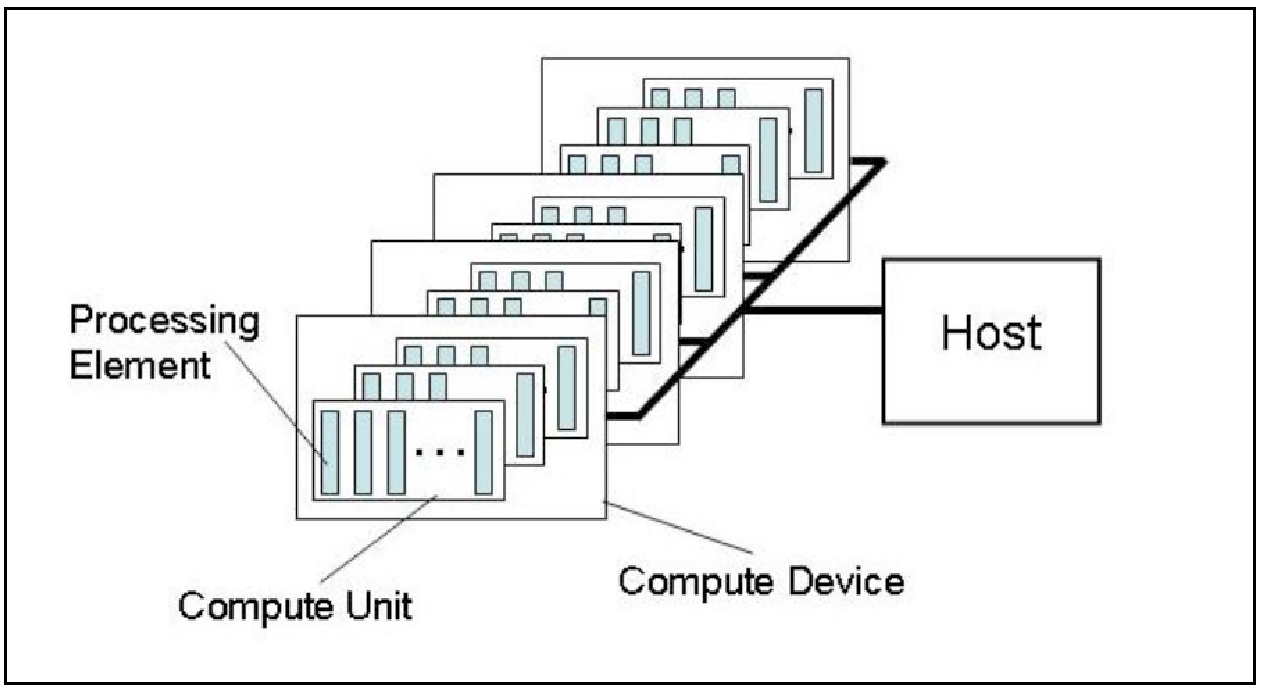
\includegraphics[width=0.8\textwidth]{PlatformModel.jpg}
    \caption{Model urządzenia}
    \label{fig:awesome_image}
	\end{figure}
	
	\subsection{Model wykonywania}
	
	\subsubsection{Zadania hosta}
	Kluczowymi częściami modelu wykonywania OpenCL są aplikacja kliencka (uruchamiana na hoście) oraz jądra (ang. kernels), które sąuruchamiane na docelowym urządzeniu wspierającym OpenCL. Głównymi zadaniami hosta są:
	\begin{itemize} 
	\item komunikacja z urządzeniem OpenCL
	\item pytanie o dostępne zasoby i cechy urządzenia
	\item tworzenie kontekstu (ang. context) (składającego się m.in. z konkretnego urządzenia (na przykład GPU) na konkretnej platformie (na przykład AMD oraz kolejki wykonywania (and. command queue))
	\item budowanie jąder i zarządzanie ich uruchamianiem
	\end{itemize}
	
	\subsubsection{Uruchamianie jąder}
	Uruchamianie jąder polega na wywołaniu odpowiedniej funkcji po stronie hosta, która kolejkuje jądro w kolejce wykonywania. Przy wywoływaniu funkcji należy wyspecyfikować jak pogrupowane w grupy robocze (ang. work group) będą jądra przy wykonywaniu, poprzez zdefiniowane N-wymiarowego zakresu (ang. NDRange), gdzie N jest nie mniejsze niż 1 i nie większe niż 3. Każdemy jądru przy instancjowaniu przypisane zostaje N indeksów. Instancja jądra jest nazywana elementem roboczym (ang. work item). Każda instancja jądra jest świadoma takich swoich parametrów jak globalny identyfikator, lokalny identyfikator czy identyfikator grupy lokalnej.
	
	
	\begin{figure}
	\centering
		\begin{subfigure}[b]{\textwidth}
			\centering
			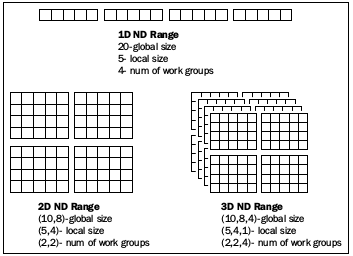
\includegraphics[width=0.8\textwidth]{ndrange.png}
			\caption{NDRange - przykłady}
			\label{fig:ndrange_examples}
		\end{subfigure}
		\begin{subfigure}[b]{\textwidth}
			\centering
			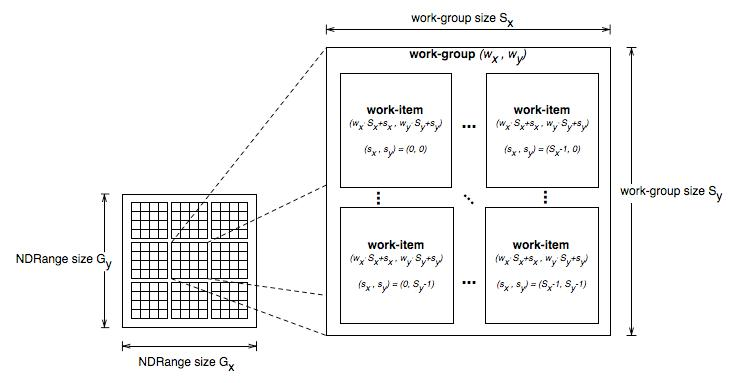
\includegraphics[width=\textwidth]{ndrange2.jpg}
			\caption{NDRange - numeracja}
			\label{fig:ndrange_numbering}
		\end{subfigure}
		\caption{NDRange}
	\end{figure}
	
	\clearpage
	\subsubsection{Kontekst OpenCL}
		Kontekst definiuje całe środowisko środowisko OpenCL czyli urządzenie, obiekty programów, jądra, obiekty pamięciowe (ang. memory objects), kolejkę wykonywania etc. Może być powiązany z jednym lub wieloma urządzeniami, ale jądra może być kolejkowany tylko jeśli odpowiada mu ten sam kontekst co danej kolejce.
		Tworzenie kontekstu polega na odpytaniu systemu o dostępne instalacje OpenCL w celu uzyskania listy platform (odpowiadających często producentom urządzeń dostępnych w komputerze). Następnie na wybranej platformie inicjalizujemy OpenCL po czym przypisujemy urządzenia do kontekstu i tworzymy na urządzeniach kolejki wykonywania.
		
	\subsubsection{Kolejka wykonywania}
	Kolejka wykonywania jest obiektem na którym komendy OpenCL są kolejkowane w celu bycia wykonanym przez urządzenie. Mogą to być komendy, które kolejkują pewną ilość jąder, ale też komendy do odczytywania danych z urządzenia czy do synchronizacji poprzez zaczekanie na zakończenie wykonywania pewnych jąder.
	
	\subsection{Model pamięci}
	
	Model pamięci w OpenCL definiuje cztery rodzaje pamięci. Do każdego z nich elementy robocze mogą uzyskać dostęp podczas wykonywania jądra. 
	
	\paragraph{Pamięć globalna}\ \\
		Na każdym urządzeniu jest to najobszerniejszy rodzaj pamięci. Każdy element roboczy w każdej grupie roboczej ma dostęp do pamięci globalnej. Słowo kluczowe \_\_global definiuje ten region. W porównaniu do pozostałych rodzajów pamięci dostęp do pamięci globalnej bywa kosztowny.
	\paragraph{Pamięć stała}\ \\
		Jest to region pamięci w urządzeniu OpenCL, który jest inicjalizowany przez hosta i jest niezmienny przez cały czas wykonywania się jądra. Słowo kluczowe \_\_constant definiuje ten region.
	\paragraph{Pamięć lokalna}\ \\
		Każdy element roboczy w grupie roboczej może używać pamięci lokalnej. Pamięć ta jest widoczna tylko w ramach danej grupy roboczej więc zapisy do pamięci przez element roboczy nie będą widoczne w innych grupach roboczych niż jego własna. Wynika to z tego, że każdy element roboczy działa na pojedynczej jednostce obliczeniowej, na której jest przechowywana ta pamięć. Słowo kluczowe \_\_local definiuje ten region.
	\paragraph{Pamięć prywatna}\ \\
		Jest to domyślny rodzaj pamięci przy tworzeniu dowolnej lokalnej zmiennej w jądrze. Zmienne te nie są widoczne w żadnych innych elementach roboczych.
	
	\subsection{Model programowania}
	Aby umożliwić wieloplatformowość każde urządzenie wspierające OpenCL powinno być zgodne z standardem OpenCL C. Jest to język bazowany na standardzie C99 w składni. Posiada on duże ilości udogodnień w zakresie arytmetyki wektorowej i macierzowej jak również duże ilości wbudowanych funkcji matematycznych.
	
	Przykładowe jądro napisane w OpenCL C wygląda nasępująco:
	
	\begin{lstlisting}
	__kernel void example_kernel(,
		float f,
		__local float* l_Array,
		__global float* g_Array)
	{
		int i = get_global_id(0);
		g_Array[i] = i;
	}
	\end{lstlisting}
	
	Widać tu znaczne podobieństwo do klasycznego C. Słowo kluczowe \_\_kernel oznacza, że funkcja jest jądrem, które może zostać uruchomione przez hosta. Słowa kluczowe \_\_local i \_\_global mówią nam o tym do jakiego rodzaju pamięci odwołują się zmienne l\_Array i g\_Array.

\section{Struktura projektu}

	\subsection{Wstęp}
		Poniższy słowny opis przedstawia główne cechy i decyzje architektoniczne, nie zagłębiając się w szczegóły dotyczące różnego rodzaju implementacji interfejsów, czy wszystkich klas wykorzystanych w projekcie. Z punkty widzenia dostarczenia funkcjonalności zgodnych z tematem pracy inżynierskiej, duża część napisanego kodu jest nieistotna. Kod ten stanowi pewnego rodzaju próbę włączenia implementacji SPH do projektu zbliżonego architektonicznie do przeciętnej gry komputerowej. Dokładny opis zastosowanej architektury, na której się wzorowaliśmy, można znaleźć w pozycji [2] z bibliografii. Różnice wynikają głównie z zastosowania innych bibliotek do osiągnięcia tych samych celów (WinAPI vs GLFW, OpenGL vs DirectX, Boost.Signals2 vs Fastdelegate etc.), oraz z tego, że w [2] opisany jest dużo bardziej złożony system niż ten zaimplementowany w naszej pracy inżynierskiej.
	
	\subsection{Kluczowe elementy stworzonego frameworku}
		\subsubsection{Obsługa OpenGL i okna}
			Klasa OpenGLSystem zajmuje się inicjalizacją okna oraz dostarczaniem informacji na temat kontekstu OpenGL, które są niezbędne do poprawnej inicjalizacji urządzenia OpenCL. Istnieje bowiem możliwość, że system OpenCL zostałby zainicjalizowany na urządzeniu innym niż OpenGL przez co niemożliwa byłaby komunikacja z wykorzystaniem OpenCL\\OpenGL interop.
			
			Klasa Window oraz klasa InputManager stanowią wrapper na funkcjonalności biblioteki GLFW. Umożliwiają one inicjalizację okna oraz obsługę zdarzeń wywołanych przez użytkownika takich jak naciśnięcie klawisza czy ruch myszką. 
			
		\subsubsection{Obsługa OpenCL}
			Klasa OpenCLSystem stanowi lekki wrapper na wszystkie konieczne funkcje OpenCL takie jak:
			\begin{itemize}
				\item Wykrywanie urządzenia, na którym jest zainicjalizowany OpenGL
				\item Tworzenie kontekstu OpenCL
				\item Czytanie i budowanie jąder OpenCL
			\end{itemize}
			W kodzie funkcjie OpenCL przeważnie są wywoływane bezpośrednio, jako że API OpenCL jest klasycznym API w języku C, które przechowuje wewnętrznie swój własny stan.
			
		\subsubsection{Obsługa zdarzeń}
			Klasa EventManager wraz z interfejsem IEventData oraz typem wyliczeniowym EventType stanowią trzon systemu zdarzeń w stworzonym frameworku. Ideą tego systemu jest to, że każda klasa może się zarejestrować na odbiór pewnego rodzaju eventów oraz sama wysłać event do systemu. Klasa EventManager jest przez to globalna dla całej aplikacji. W każdej klatce zdarzenia, które wystąpiły są wysyłane do opowiednich odbiorców.
			
			Dzięki tej klasie osiągamy inwersję zależności (dependency inversion). Poszczególne obiekty systemu nie muszę wiedzieć o żadnych innych obiektach. Chcąc poinformować, że zaszło jakieś zdarzenie lub chcąc wysłać jakąś wiadomość do systemu jedyne co obiekty muszą posiadać to referencję do EventManager'a. To on zajmuje się dystrybucją wiadomości do zainteresowanych odbiorców.
		 
		\subsubsection{Model actorów złożonych z komponentów}
		
			W każdej grze istnieje koncepja aktorów (zwanych czasami obiektami gry (and. game object)), które mogą wykonywać jakieś akcje w czasie, posiadają logikę rysowania, przechowują swój stan i położenie. Klasyczne podejście do budowy tego typu obiektów - wszystko w jednej klasie - łamie SRP (Single Responsibility Principle). Postanowiliśmy więc wykorzystać model zwany CBSE (Component-Based Software Engineering) do reprezentacji aktorów. 
			
			Każdy aktor składa się z wielu komponentów definujących takie rzeczy jak logikę, sposób rysowania, przemieszczenie w przestrzeni. Mogą też istnieć specyficzne komponenty takie jak komponent kamery. Jako, że każdy komponent zajmuje się swoją własną dziedziną nie jest łamane SRP i system staje się znacząco bardziej skalowalny. 
			
			Przykładem zastosowania tego modelu są klasy WaterLogicComponent, WaterModelComponent oraz WaterRenderComponent - każda z nich zajmuje się dostarczeniem jednej funkcjonalności. WaterLogiComponent zawiera logikę OpenCL, która porusza modelem płynu zdefiniowanym i zainicjalizowanym w WaterModelComponent. WaterRenderComponent natomiast komunikuje się z WaterModelComponent w celu wyświetlenia modelu cieczy na ekranie. Łatwym byłoby stworzenie innego sposoby renderowania czy innego zachowania cieczy (co było wykonywane w pierwszych iteracjach) i polegałoby tylko na podmianie tych, raczej lekkich, komponentów.
			
		\subsubsection{Wykorzystanie C++11}
		
		Pisząc kod stosowaliśmy się do idiomu C++ RAII (Resource Acquisition Is Initialization). W całym kodzie słowo kluczowe "delete" nie występuje ponieważ wszystkie zmienne są inicjalizowane w taki sposób, aby kiedy nie są potrzebne same się usuwały. Wykorzystujemy do tego takie dodatki w C++11 jak shared\_ptr, unique\_ptr czy std::array zamist zwykłych wskaźników i wskaźników na tablice. Korzystamy też z nowowprowadzonych lambd oraz słowa kluczowego auto.

\section{Sposób implementacji metody SPH}
Nasza implementacja metody SPH składa się z 9 jąder i wykorzystujemy 10 globalnych buforów. Dodatkowo korzystamy z biblioteki clpp, która dostarcza nam optymalnych implementacji sortowań na kartę graficzną algorytmem Radix Sort.
		
		\subsection{Wyszukanie sąsiadów cel}
			\paragraph{Nazwa jądra} \ \\
				find\_voxel\_neighbours
			\paragraph{Dane wejściowe} \ \\
					\begin{tabular}{| p{\dimexpr 0.25\linewidth-2\tabcolsep} | p{\dimexpr 0.10\linewidth-2\tabcolsep} | p{\dimexpr 0.20\linewidth-2\tabcolsep} | p{\dimexpr 0.45\linewidth-2\tabcolsep} |}
					\hline
						Nazwa & Typ & Rozmiar & Opis \\
					\hline
						lbf (left bottom front)& float4 & 1 & Wierzchołek definiujący pudło obliczeniowe \\ 
					\hline
						rtb (right top back) & float4 & 1 & Wierzchołek definiujący pudło obliczeniowe  \\ 
					\hline
						h & float & 1 & Promień wygładzania \\ 
					\hline
    				\end{tabular}
			\paragraph{Dane wyjściowe} \ \\
				\begin{tabular}{| p{\dimexpr 0.25\linewidth-2\tabcolsep} | p{\dimexpr 0.10\linewidth-2\tabcolsep} | p{\dimexpr 0.20\linewidth-2\tabcolsep} | p{\dimexpr 0.45\linewidth-2\tabcolsep} |}
				\hline
					Nazwa & Typ & Rozmiar & Opis \\
				\hline
					voxel\_neighbour\_map & int & 64 ${\cdot}$ ilość cel & Sąsiedzi dla każdej celi \\ 
				\hline
				\end{tabular}
			\paragraph{Dane wywoływania} \ \\
					\begin{tabular}{| p{\dimexpr 0.20\linewidth-2\tabcolsep} | p{\dimexpr 0.40\linewidth-2\tabcolsep} | p{\dimexpr 0.40\linewidth-2\tabcolsep}|}
					\hline
						Ilość jąder & Ilość grup lokalnych & Ilość elementów w grupie lokalnej \\
					\hline
						Ilość cel & n/d & n/d \\ 
					\hline
    				\end{tabular}
			\paragraph{Opis} \ \\
				\indent Każdą celę dzielimy na 8 równych części i dla każdej z tych części znajdujemy 8 sąsiadujących cel (w tym obecną). Informacja ta jest potrzebna przy wyszukiwaniu sąsiadów w późniejszej części algorytmu. Kluczowe jest w tym algorytmie uwzględnienie warunkówa brzegowych. W naszej implementacji wykorzystaliśmy tzw. periodyczne warunki przegowe, które sprawiają że na brzegach wyszukiwanie sąsiadów jest zawijane na drugą stronę pudła obliczeniowego, kiedy za nie wyjdziemy.
				
		\subsection{Przypisanie cząstek do cel}
			\paragraph{Nazwa jądra} \ \\
				hash\_particles
			\paragraph{Dane wejściowe} \ \\
				\begin{tabular}{| p{\dimexpr 0.25\linewidth-2\tabcolsep} | p{\dimexpr 0.10\linewidth-2\tabcolsep} | p{\dimexpr 0.20\linewidth-2\tabcolsep} | p{\dimexpr 0.45\linewidth-2\tabcolsep} |}
				\hline
					Nazwa & Typ & Rozmiar & Opis \\
				\hline
					lbf (left bottom front)& float4 & 1 & Wierzchołek definiujący pudło obliczeniowe \\ 
				\hline
					rtb (right top back) & float4 & 1 & Wierzchołek definiujący pudło obliczeniowe  \\ 
				\hline
					h & float & 1 & Promień wygładzania \\ 
				\hline
					position & float4 & ilość cząstek & Pozycje cząstek \\
				\hline
				\end{tabular}
			\paragraph{Dane wyjściowe} \ \\
				\begin{tabular}{| p{\dimexpr 0.25\linewidth-2\tabcolsep} | p{\dimexpr 0.10\linewidth-2\tabcolsep} | p{\dimexpr 0.20\linewidth-2\tabcolsep} | p{\dimexpr 0.45\linewidth-2\tabcolsep} |}
				\hline
					Nazwa & Typ & Rozmiar & Opis \\
				\hline
					voxel\_particle & int2 & ilość cząstek & Mapa zawierająca przypisania cząstek do cel \\ 
				\hline
				\end{tabular}
			\paragraph{Dane wywoływania} \ \\
				\begin{tabular}{| p{\dimexpr 0.20\linewidth-2\tabcolsep} | p{\dimexpr 0.40\linewidth-2\tabcolsep} | p{\dimexpr 0.40\linewidth-2\tabcolsep}|}
				\hline
					Ilość jąder & Ilość grup lokalnych & Ilość elementów w grupie lokalnej \\
				\hline
					Ilość cząstek & n/d & n/d \\ 
				\hline
				\end{tabular}
			\paragraph{Opis} \ \\
				\indent Dla każdej cząstki obliczamy w jakiej celi się znajduje i tę informację zapisujemy s buforze voxel\_particle,
		\subsection{Sortowanie cząstek}
			\subsubsection{Biblioteka clpp}
			\paragraph{Dane wejściowe} \ \\
				\begin{tabular}{| p{\dimexpr 0.25\linewidth-2\tabcolsep} | p{\dimexpr 0.10\linewidth-2\tabcolsep} | p{\dimexpr 0.20\linewidth-2\tabcolsep} | p{\dimexpr 0.45\linewidth-2\tabcolsep} |}
				\hline
					Nazwa & Typ & Rozmiar & Opis \\
				\hline
					voxel\_particle & int2 & ilość cząstek & Mapa zawierająca przypisania cząstek do cel \\ 
				\hline
				\end{tabular}
			\paragraph{Dane wyjściowe} \ \\
				\begin{tabular}{| p{\dimexpr 0.25\linewidth-2\tabcolsep} | p{\dimexpr 0.10\linewidth-2\tabcolsep} | p{\dimexpr 0.20\linewidth-2\tabcolsep} | p{\dimexpr 0.45\linewidth-2\tabcolsep} |}
				\hline
					Nazwa & Typ & Rozmiar & Opis \\
				\hline
					voxel\_particle & int2 & ilość cząstek & Mapa zawierająca posortowane po numerze celi przypisania cząstek do cel\\ 
				\hline
				\end{tabular}
			\paragraph{Opis} \ \\
				\indent Wykorzystaliśmy zewnętrzną bibliotekę clpp w celu posortowania danych znajdujących się w buforze voxel\_particle po numerze celi (początkowo są posortowane po numerze cząstki).
			\subsubsection{Dodatkowe operacje po sortowaniu}
				\paragraph{Nazwa jądra} \ \\
					sort\_post\_pass
				\paragraph{Dane wejściowe} \ \\
					\begin{tabular}{| p{\dimexpr 0.25\linewidth-2\tabcolsep} | p{\dimexpr 0.10\linewidth-2\tabcolsep} | p{\dimexpr 0.20\linewidth-2\tabcolsep} | p{\dimexpr 0.45\linewidth-2\tabcolsep} |}
					\hline
						Nazwa & Typ & Rozmiar & Opis \\
					\hline
						velocity & float4 & ilość cząstek & Prędkości cząstek \\
					\hline
						position & float4 & ilość cząstek & Pozycje cząstek \\
					\hline
					\end{tabular}
				\paragraph{Dane wyjściowe} \ \\
					\begin{tabular}{| p{\dimexpr 0.25\linewidth-2\tabcolsep} | p{\dimexpr 0.10\linewidth-2\tabcolsep} | p{\dimexpr 0.20\linewidth-2\tabcolsep} | p{\dimexpr 0.45\linewidth-2\tabcolsep} |}
					\hline
						Nazwa & Typ & Rozmiar & Opis \\
					\hline
						sorted\_velocity & float4 & ilość cząstek & Prędkości cząstek posortowane jak voxel\_particle\\
					\hline
						sorted\_position & float4 & ilość cząstek & Pozycje cząstek posortowane jak voxel\_particle\\
					\hline
					\end{tabular}
				\paragraph{Dane wywoływania} \ \\
					\begin{tabular}{| p{\dimexpr 0.20\linewidth-2\tabcolsep} | p{\dimexpr 0.40\linewidth-2\tabcolsep} | p{\dimexpr 0.40\linewidth-2\tabcolsep}|}
					\hline
						Ilość jąder & Ilość grup lokalnych & Ilość elementów w grupie lokalnej \\
					\hline
						Ilość cząstek & n/d & n/d \\ 
					\hline
					\end{tabular}
				\paragraph{Opis} \ \\
					\indent Po posortowaniu voxel\_particle konieczne jest przepisanie buforu pozycji i buforu prędkości tak, aby były w tej samej kolejności co voxel\_particle.
		\subsection{Indeksowanie cząstek}
			\subsubsection{Funkcja indeksująca}
				\paragraph{Nazwa jądra} \ \\
					find\_index
				\paragraph{Dane wejściowe} \ \\
					\begin{tabular}{| p{\dimexpr 0.25\linewidth-2\tabcolsep} | p{\dimexpr 0.10\linewidth-2\tabcolsep} | p{\dimexpr 0.20\linewidth-2\tabcolsep} | p{\dimexpr 0.45\linewidth-2\tabcolsep} |}
					\hline
						Nazwa & Typ & Rozmiar & Opis \\
					\hline
						voxel\_particle & int2 & ilość cząstek & Mapa zawierająca przypisania cząstek do cel \\ 
					\hline
						particle\_count & int & ilość cząstek & Ilość cząstek \\
					\hline
					\end{tabular}
				\paragraph{Dane wyjściowe} \ \\
					\begin{tabular}{| p{\dimexpr 0.25\linewidth-2\tabcolsep} | p{\dimexpr 0.10\linewidth-2\tabcolsep} | p{\dimexpr 0.20\linewidth-2\tabcolsep} | p{\dimexpr 0.45\linewidth-2\tabcolsep} |}
					\hline
						Nazwa & Typ & Rozmiar & Opis \\
					\hline
						grid\_cell\_index & int & ilość cel & Indeksy początków danych dla każdej celi w tablicy voxel\_particle \\
					\hline
				\end{tabular}
				\paragraph{Dane wywoływania} \ \\
					\begin{tabular}{| p{\dimexpr 0.20\linewidth-2\tabcolsep} | p{\dimexpr 0.40\linewidth-2\tabcolsep} | p{\dimexpr 0.40\linewidth-2\tabcolsep}|}
					\hline
						Ilość jąder & Ilość grup lokalnych & Ilość elementów w grupie lokalnej \\
					\hline
						Ilość cel & n/d & n/d \\ 
					\hline
					\end{tabular}
				\paragraph{Opis} \ \\
					\indent W dalszej części algorytmu będziemy korzystać z informacji o początku danych dla danej celi w tablicach sorted\_position, sorted\_velocity i voxel\_particle. Znajdujemy je więc w osobnym jądrze i zapisujemy do bufora grid\_cell\_index.
					
			\subsubsection{Dodatkowe operacje po indeksowaniu}
				\paragraph{Nazwa jądra} \ \\
					index\_post\_pass
				\paragraph{Dane wejściowe} \ \\
					\begin{tabular}{| p{\dimexpr 0.25\linewidth-2\tabcolsep} | p{\dimexpr 0.10\linewidth-2\tabcolsep} | p{\dimexpr 0.20\linewidth-2\tabcolsep} | p{\dimexpr 0.45\linewidth-2\tabcolsep} |}
					\hline
						Nazwa & Typ & Rozmiar & Opis \\
					\hline
						grid\_cell\_index & int & ilość cel & Indeksy początków danych dla każdej celi w tablicy voxel\_particle \\
					\hline
				\end{tabular}
				\paragraph{Dane wyjściowe} \ \\
					\begin{tabular}{| p{\dimexpr 0.25\linewidth-2\tabcolsep} | p{\dimexpr 0.10\linewidth-2\tabcolsep} | p{\dimexpr 0.20\linewidth-2\tabcolsep} | p{\dimexpr 0.45\linewidth-2\tabcolsep} |}
					\hline
						Nazwa & Typ & Rozmiar & Opis \\
					\hline
						grid\_cell\_index & int & ilość cel & Indeksy początków danych dla każdej celi w tablicy voxel\_particle \\
					\hline
				\end{tabular}
				\paragraph{Dane wywoływania} \ \\
					\begin{tabular}{| p{\dimexpr 0.20\linewidth-2\tabcolsep} | p{\dimexpr 0.40\linewidth-2\tabcolsep} | p{\dimexpr 0.40\linewidth-2\tabcolsep}|}
					\hline
						Ilość jąder & Ilość grup lokalnych & Ilość elementów w grupie lokalnej \\
					\hline
						Ilość cel & n/d & n/d \\ 
					\hline
					\end{tabular}
				\paragraph{Opis} \ \\
					\indent Dla niektórych cel po kroku index nie zostaną znalezione poprawne wartości, w przypadku kiedy cela jest pusta. Jądro index\_post\_pass przepisuje informacje z kolejnej niepustej celi przez co mimo puste cele nie przeszkadzają w algorytmie w dalszych krokach.
					
		\subsection{Znajdowanie sąsiadów cząstek}
			\paragraph{Nazwa jądra} \ \\
					neighbour\_map
				\paragraph{Dane wejściowe} \ \\
					\begin{tabular}{| p{\dimexpr 0.25\linewidth-2\tabcolsep} | p{\dimexpr 0.10\linewidth-2\tabcolsep} | p{\dimexpr 0.20\linewidth-2\tabcolsep} | p{\dimexpr 0.45\linewidth-2\tabcolsep} |}
					\hline
						Nazwa & Typ & Rozmiar & Opis \\
					\hline
						voxel\_particle & int2 & ilość cząstek & Mapa zawierająca przypisania cząstek do cel \\ 
					\hline
						grid\_cell\_index & int & ilość cel & Indeksy początków danych dla każdej celi w tablicy voxel\_particle \\
					\hline
						sorted\_position & float4 & ilość cząstek & Pozycje cząstek posortowane jak voxel\_particle\\
					\hline
						voxel\_neighbour\_map & int & 64 ${\cdot}$ ilość cel & Sąsiedzi dla każdej celi \\ 
					\hline
						neighbours\_to\_find & int & 1 & Ilość sąsiadów, którą chcemy znaleźć dla każdej cząstki \\ 
					\hline
						lbf (left bottom front)& float4 & 1 & Wierzchołek definiujący pudło obliczeniowe \\ 
					\hline
						rtb (right top back) & float4 & 1 & Wierzchołek definiujący pudło obliczeniowe  \\ 
					\hline
						h & float & 1 & Promień wygładzania \\ 
					\hline	
				\end{tabular}
				\paragraph{Dane wyjściowe} \ \\
					\begin{tabular}{| p{\dimexpr 0.25\linewidth-2\tabcolsep} | p{\dimexpr 0.10\linewidth-2\tabcolsep} | p{\dimexpr 0.20\linewidth-2\tabcolsep} | p{\dimexpr 0.45\linewidth-2\tabcolsep} |}
					\hline
						Nazwa & Typ & Rozmiar & Opis \\
					\hline
						neighbour\_map & int & neighbours\_to\_find ${\cdot}$ ilość cząstek & Mapa sąsiadów każdej cząstki\\
					\hline
				\end{tabular}
				\paragraph{Dane wywoływania} \ \\
					\begin{tabular}{| p{\dimexpr 0.20\linewidth-2\tabcolsep} | p{\dimexpr 0.40\linewidth-2\tabcolsep} | p{\dimexpr 0.40\linewidth-2\tabcolsep}|}
					\hline
						Ilość jąder & Ilość grup lokalnych & Ilość elementów w grupie lokalnej \\
					\hline
						Ilość cząstek & n/d & n/d \\ 
					\hline
					\end{tabular}
				\paragraph{Opis} \ \\
					\indent Dla każdej cząstki wyszukujemy pewną, definiowaną w programie, ilość sąsiadów. Są to cząstki z którymi będziemy obliczać interakcje w następnych krokach.
 
		\subsection{Obliczenie gęstości i ciśnienia}
				\paragraph{Nazwa jądra} \ \\
					compute\_density\_pressure
				\paragraph{Dane wejściowe} \ \\
					\begin{tabular}{| p{\dimexpr 0.25\linewidth-2\tabcolsep} | p{\dimexpr 0.10\linewidth-2\tabcolsep} | p{\dimexpr 0.20\linewidth-2\tabcolsep} | p{\dimexpr 0.45\linewidth-2\tabcolsep} |}
					\hline
						Nazwa & Typ & Rozmiar & Opis \\
					\hline
						sorted\_position & float4 & ilość cząstek & Pozycje cząstek posortowane jak voxel\_particle\\
					\hline
						neighbour\_map & int & neighbours\_to\_find ${\cdot}$ ilość cząstek & Mapa sąsiadów każdej cząstki\\
					\hline
						neighbours\_to\_find & int & 1 & Ilość sąsiadów, którą chcemy znaleźć dla każdej cząstki \\ 
					\hline
						m & float & 1 & Masa cząstki \\ 
					\hline
						h & float & 1 & Promień wygładzania \\ 
					\hline
						k & float & 1 & Stała przed nawiasem w równaniu stanu \\ 
					\hline
						${\rho_0}$ & float & 1 & Gęstość w stanie równowagi \\ 
					\hline	
				\end{tabular}
				\paragraph{Dane wyjściowe} \ \\
					\begin{tabular}{| p{\dimexpr 0.25\linewidth-2\tabcolsep} | p{\dimexpr 0.10\linewidth-2\tabcolsep} | p{\dimexpr 0.20\linewidth-2\tabcolsep} | p{\dimexpr 0.45\linewidth-2\tabcolsep} |}
					\hline
						Nazwa & Typ & Rozmiar & Opis \\
					\hline
						density\_and\_pressure & float2 & ilość cząstek & Gęstość i ciśnienie dla każdej cząstki\\
					\hline
				\end{tabular}
				\paragraph{Dane wywoływania} \ \\
					\begin{tabular}{| p{\dimexpr 0.20\linewidth-2\tabcolsep} | p{\dimexpr 0.40\linewidth-2\tabcolsep} | p{\dimexpr 0.40\linewidth-2\tabcolsep}|}
					\hline
						Ilość jąder & Ilość grup lokalnych & Ilość elementów w grupie lokalnej \\
					\hline
						Ilość cząstek & Ilość cząstek / ilość sąsiadów & Ilość sąsiadów \\ 
					\hline
					\end{tabular}
				\paragraph{Opis} \ \\
					\indent Dla każdej cząstki, korzystając z listy sąsiadów, wzoru na gęstość i równania stanu obliczamy gęstość a następnie ciśnienie. 
		\subsection{Obliczanie przyspieszenia}
				\paragraph{Nazwa jądra} \ \\
					compute\_acceleration
				\paragraph{Dane wejściowe} \ \\
					\begin{tabular}{| p{\dimexpr 0.25\linewidth-2\tabcolsep} | p{\dimexpr 0.10\linewidth-2\tabcolsep} | p{\dimexpr 0.20\linewidth-2\tabcolsep} | p{\dimexpr 0.45\linewidth-2\tabcolsep} |}
					\hline
						Nazwa & Typ & Rozmiar & Opis \\
					\hline
						sorted\_position & float4 & ilość cząstek & Pozycje cząstek posortowane jak voxel\_particle\\
					\hline
						sorted\_velocity & float4 & ilość cząstek & Prędkości cząstek posortowane jak voxel\_particle\\
					\hline
						density\_and\_pressure & float2 & ilość cząstek & Gęstość i ciśnienie dla każdej cząstki\\
					\hline
						neighbour\_map & int & neighbours\_to\_find ${\cdot}$ ilość cząstek & Mapa sąsiadów każdej cząstki\\
					\hline
						g & float & 1 & Przyspieszenie grawitacyjne \\ 
					\hline
						m & float & 1 & Masa cząstki \\ 
					\hline
						h & float & 1 & Promień wygładzania \\ 
					\hline	
				\end{tabular}
				\paragraph{Dane wyjściowe} \ \\
					\begin{tabular}{| p{\dimexpr 0.25\linewidth-2\tabcolsep} | p{\dimexpr 0.10\linewidth-2\tabcolsep} | p{\dimexpr 0.20\linewidth-2\tabcolsep} | p{\dimexpr 0.45\linewidth-2\tabcolsep} |}
					\hline
						Nazwa & Typ & Rozmiar & Opis \\
					\hline
						acceleration & float4 & ilość cząstek & Wektor przyspieszenia dla każdej cząstki\\
					\hline
				\end{tabular}
				\paragraph{Dane wywoływania} \ \\
					\begin{tabular}{| p{\dimexpr 0.20\linewidth-2\tabcolsep} | p{\dimexpr 0.40\linewidth-2\tabcolsep} | p{\dimexpr 0.40\linewidth-2\tabcolsep}|}
					\hline
						Ilość jąder & Ilość grup lokalnych & Ilość elementów w grupie lokalnej \\
					\hline
						Ilość cząstek & Ilość cząstek / ilość sąsiadów & Ilość sąsiadów \\ 
					\hline
					\end{tabular}
				\paragraph{Opis} \ \\
					\indent Dla każdej cząstki obliczamy przyspieszenie korzystając z wzorów opisanych w dokumentacji użytkownika w sekcji 1.
		\subsection{Wykonanie kroku czasowego}
				\paragraph{Nazwa jądra} \ \\
					integrate
				\paragraph{Dane wejściowe} \ \\
					\begin{tabular}{| p{\dimexpr 0.25\linewidth-2\tabcolsep} | p{\dimexpr 0.10\linewidth-2\tabcolsep} | p{\dimexpr 0.20\linewidth-2\tabcolsep} | p{\dimexpr 0.45\linewidth-2\tabcolsep} |}
					\hline
						Nazwa & Typ & Rozmiar & Opis \\
					\hline
						position & float4 & ilość cząstek & Pozycje cząstek \\
					\hline
						velocity & float4 & ilość cząstek & Prędkości cząstek \\
					\hline
						density\_and\_pressure & float2 & ilość cząstek & Gęstość i ciśnienie dla każdej cząstki\\
					\hline
						delta\_time & float & 1 & Czas, który minął od poprzedniej klatki symulacji \\ 
					\hline
						lbf (left bottom front)& float4 & 1 & Wierzchołek definiujący pudło obliczeniowe \\ 
					\hline
						rtb (right top back) & float4 & 1 & Wierzchołek definiujący pudło obliczeniowe  \\ 
					\hline
				\end{tabular}
				\paragraph{Dane wyjściowe} \ \\
					\begin{tabular}{| p{\dimexpr 0.25\linewidth-2\tabcolsep} | p{\dimexpr 0.10\linewidth-2\tabcolsep} | p{\dimexpr 0.20\linewidth-2\tabcolsep} | p{\dimexpr 0.45\linewidth-2\tabcolsep} |}
					\hline
						Nazwa & Typ & Rozmiar & Opis \\
					\hline
						velocity & float4 & ilość cząstek & Prędkości cząstek - zmienione \\
					\hline
				\end{tabular}
				\paragraph{Dane wywoływania} \ \\
					\begin{tabular}{| p{\dimexpr 0.20\linewidth-2\tabcolsep} | p{\dimexpr 0.40\linewidth-2\tabcolsep} | p{\dimexpr 0.40\linewidth-2\tabcolsep}|}
					\hline
						Ilość jąder & Ilość grup lokalnych & Ilość elementów w grupie lokalnej \\
					\hline
						Ilość cząstek & n/d & n/d \\ 
					\hline
					\end{tabular}
				\paragraph{Opis} \ \\
					\indent Zgodnie z policzonym w poprzednim kroku przyspieszeniem, obliczamy nową prędkość a następnie pozycję każdej z cząstek. Ważnym jest aby nie pozwolić cząstkom uciec z pudła obliczeniowego. Kiedy zachodzi taka sytuacja odbijamy cząstkę od ściany zmieniając jej wektor prędkości i pozycję.
					
		\subsection{Podsumowanie}
		
			\noindent Końcowy przebieg algorytmu wygląda następująco:
			\ \\
			\ \\
			\begin{tabular}{| p{\dimexpr 0.25\linewidth-2\tabcolsep} | p{\dimexpr 0.75\linewidth-2\tabcolsep} |}
				\hline
					find\_voxel\_neighbours & Znalezienie sąsiadów dla każdej celi \\
				\hline
					hash\_particles & Przypisanie cząstek do cel \\
				\hline
					clpp\_sort & Posortowanie mapowania z czątki na celę aby zamieniło się w mapowanie celi na cząstkę\\
				\hline
					sort\_post\_pass & Przepisanie buforów position i velocity by były w kolejności posortowanej\\
				\hline
					find\_index & Znalezienie indeksów w których zaczynają się informacje na temat danych cel \\
				\hline
					index\_post\_pass & Poprawa indeksów dla cel, które nie mają cząstek \\
				\hline
					neighbour\_map & Znalezienie sąsiadów dla każdej cząstki \\
				\hline
					compute\_density \_pressure & Obliczenie gęstości i ciśnienia \\
				\hline
					compute\_acceleration & Obliczenie przyspieszenia \\
				\hline
					integrate & Krok czasowy \\
				\hline
			\end{tabular}
			
			\ \\
			\ \\
			Do implementacji zostały wykorzystane następujące globalne bufory:
			\ \\
			\begin{tabular}{| p{\dimexpr 0.25\linewidth-2\tabcolsep} | p{\dimexpr 0.25\linewidth-2\tabcolsep} | p{\dimexpr 0.50\linewidth-2\tabcolsep} |}
				\hline
					position & float4[ilość cząstek] & Pozycje cząstek - bufor ten jest współdzielony z OpenGL i jest wykorzystywany do wizualizacji cząstek. \\
				\hline
					velocity & float4[ilość cząstek] & Prędkości cząstek \\
				\hline
					acceleration & float4[ilość cząstek] & Wektor przyspieszenia dla każdej cząstki\\
				\hline
					grid\_cell\_index & int[ilość cel] & Indeksy początków danych dla każdej celi w tablicy voxel\_particle \\
				\hline
					voxel\_particle & int2[ilość cząstek] & Mapa zawierająca przypisania cząstek do cel \\ 
				\hline
					sorted\_position & float4[ilość cząstek] & Pozycje cząstek posortowane jak voxel\_particle\\
				\hline
					sorted\_velocity & float4[ilość cząstek] & Prędkości cząstek posortowane jak voxel\_particle\\
				\hline
					density\_and\_pressure & float2[ilość cząstek] & Gęstość i ciśnienie dla każdej cząstki\\
				\hline
					neighbour\_map & int[neighbours\_to\_find ${\cdot}$ ilość cząstek] & Mapa sąsiadów każdej cząstki\\
				\hline
					voxel\_neighbour\_map & int[64 ${\cdot}$ ilość cel] & Sąsiedzi dla każdej celi \\
				\hline
			\end{tabular}

\section{Sposób implementacji wizualizacji metody SPH}

	Do implementacji wizualizacji metody SPH wykorzystaliśmy bibliotekę OpenGL. Zdecydowaliśmy się na nią ponieważ alternatywny DirectX nie działałby na systemach unixowych, a zależało nam, aby nasza aplikacja była możliwie wieloplatformowa.
	
	\subsection{Podejście naiwne}
		Początkowo, aby renderować ciecz, dla każdej cząstki rysowaliśmy sferę o ustalonym promieniu i środku w punkcie w którym znajdowała się cząstka. Przy małych ilościach cząstek dawało to zadowalające wyniki. Sfery, które rysowaliśmy bywały kanciaste, ale nie sprawiało to większych problemów i symulacja wyglądała zadowalająco.
		
		Niestety kiedy przekroczyliśmy 1'000'000 cząstek w symulacji rysowanie sfer stało się głównym wąskim gardłem aplikacji ze względu na dużą ilość trójkątów. Jednym rozwiązaniem tego problemu byłoby zastosowanie algorytmu usuwania niewidocznych przestrzeni (ang. occlusion culling). Zdecydowaliśmy się na inne, prostsze w implementacji rozwiązanie.
		
	\subsection{Wykorzystanie bilboardów}
		Bilboardy to technika polegająca na wykorzystaniu cieniowania geometrycznego (ang. geometry shader) do wygenerowania w trakcie rysowania dodatkowych trójkątów. W naszym przypadku generowaliśmy prostokąt (2 trójkąty) zwrócony zawsze w kierunku kamery. 
		
		Następnie w trakcie cieniowania pikseli na tym bilboardzie rysowaliśmy koło. Porównanie efektów techniki naiwnej z techniką wykorzystania bilboardów można zobaczyć w rysunku \ref{fig:impostor_image}
		
		\begin{figure}[h!]
    	\centering
    	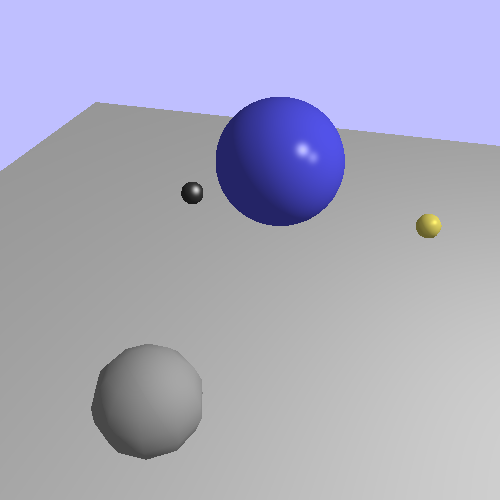
\includegraphics[width=0.8\textwidth]{impostor.png}
    	\caption{Sfera niebieska i czarna to tak naprawdę koła zwrócone w stronę kamery. Szara i żółta to sfery złożone z trójkątów w przestrzeni}
    	\label{fig:impostor_image}
		\end{figure}
		
		Uzyskany efekt wygląda znakomicie i jako, że sfery składają się tylko z 2 trójkątów, rysowanie symulowanej cieczy przestało być problemem. [ref: http://www.arcsynthesis.org/gltut/illumination/tutorial%2013.html]
		
\section{Opis wykorzystanych zewnętrznych bibliotek}

	\ \\
	\begin{tabular}{| p{\dimexpr 0.25\linewidth-2\tabcolsep} | p{\dimexpr 0.75\linewidth-2\tabcolsep} |}
		\hline
			OpenCL & Szeroki opis znajduje się w sekcji 1. \\
		\hline
			OpenGL &  Jest to specyfikacja otwartego i uniwersalnego API do tworzenia grafiki. Ciekawym resultatem "uniwersalności" bibliotek typu OpenGL i OpenCL jest to, że de facto OpenCL i OpenGL same w sobie są jedynie specyfikacjami API a nie implementacjami. W gestii producentów leży implementacja danego API na dostarczane urządzenie.\\
		\hline
			CLPP &  Jest to ogólnodostępna biblioteka do sortowania z wykorzystaniem OpenCL. Wykorzystaliśmy ją w projekcie ponieważ sortowanie było kluczowym elementem algorytmu, a clpp oferowało wysoce zoptymalizowaną, w stosunku do naszej, implementację radix sorta działająca na GPU.\\
		\hline
			GLFW &  Jest to jedna z najlżejszych wieloplatformowych bibliotek do tworzenia i obsługi okien, dostępnych w C++. W naszym projekcie klasy Window i InputManager są wrapperami na funkcjonalności GLFW. Ma ona tę wadę, że nie umożliwia łatwego wyświetlania tekstu czy prostych obiektów geometrycznych w oknie tak jak konkurencyjne biblioteki SFML, SDL czy FreeGLUT. Niemniej jednak do celów naszej aplikacji była wystarczająca. \\
		\hline
			Boost.Signals2 &  Biblioteka boost jest przez wielu uważana za drugi standard C++, oczywiśćie po libstdc++. Boost.Signals2 udostępnia funkcjonalność sygnałów i slotów, zbliżoną na przykład do systemu eventów w językach takich jak C\#. Została ona wykorzystana do stworzenia globalnego systemu zdarzeń, dzięki któremu trywialnym stało się pisanie mapowania działań użytkownika na funkcje wewnątrz programu. \\
		\hline	
	\end{tabular}
	\clearpage
	
	\nocite{OpenCLProgrammingGuide,GameCodingComplete,CLPP,SPHWebinar}
	\bibliography{bibliografia}
	
\end{document}
